\documentclass[conference]{IEEEtran}
\IEEEoverridecommandlockouts
% The preceding line is only needed to identify funding in the first footnote. If that is unneeded, please comment it out.
\usepackage{cite}
\usepackage{amsmath,amssymb,amsfonts}
\usepackage{graphicx}
\usepackage{textcomp}
\usepackage{xcolor}
\def\BibTeX{{\rm B\kern-.05em{\sc i\kern-.025em b}\kern-.08em
    T\kern-.1667em\lower.7ex\hbox{E}\kern-.125emX}}
\title{
\vspace{1cm}
{
\includegraphics[width=0.15\textwidth]{iithlogo.jpg} \\ Assembly Assignment} }
\author{Akkugari Ruchika \\ Roll No: FWC22276 \\ akkugariruchika@gmail.com}
 \begin{document}
\maketitle
 \section {ABSTRACT}
 The propagation delay of the $2 \times 1$ MUX shown in the circuit is $10ns$.Consider the propogation delay of the inverter as $0ns$. 
 \begin {figure}[h]
 \centering
 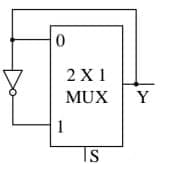
\includegraphics[width=0.35\textwidth]{as11.jpg}
 \caption{\label{fig: $2 \times 1$ MUX}}
 \end {figure}
\section{COMPONENTS}
The required components list is given in Table: I. The pin out diagram of LCD is:
 \begin{figure}[h]
	 \centering
	 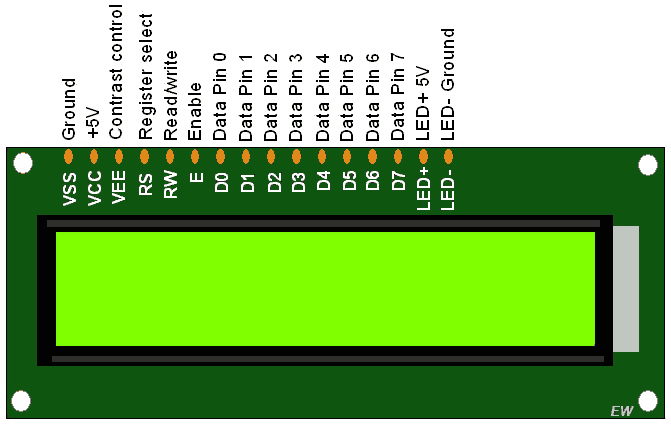
\includegraphics[width=0.35\textwidth]{lcd.png}
	 \caption{\label{fig:LCD}}
 \end{figure}
  \begin{table} [htbp]
\centering
\begin{tabular}{| c | c | c |} \hline
Components & Value & Quantity \\\hline
	LCD & $16\times2$ & 1 \\ \hline
Arduino & UNO & 1 \\ \hline
Jumper Wires &  & 20 \\ \hline
Breadboard & & 1 \\ 
\hline
\end{tabular}
\vspace{0.1cm}
\caption{\label{tab:widgets}}
\end{table}\\
\section{PROCEDURE}
In the above problem, if $S$ is set $1$ then the output $Y$ is "a square wave of frequency 50 MHz". This statement is displayed on the LCD. To display output on a $16\times2$ LCD using arduino, the LCD is connected to the arduino's digtal I/O pins. The assembly code is written to intitialize the LCD in a 4-bit mode and send ASCII characters to the display. The assembly code is compiled in Termux, generating a hex file. This pre-compiled code is dumped into the arduino, which executes the code and displays the output on the LCD. The connections between the LCD and arduino are shown in the figure 3. \\ The Truth Table for $2\times1 MUX$:
 \begin{table}[htbp]
	 \centering
	 \begin{tabular}{| c | c |}\hline
		 S  & Y\\
		 \hline
		  0 & $I_{0}$ (input 1)\\ \hline
		  1 & $I_{1}$ (input 2)\\ 
		  \hline
	 \end{tabular}
	 \vspace{0.1cm}
	 \caption{\label{tab:widgets}}
 \end{table}
 \begin{figure}[h]
	 \centering
	 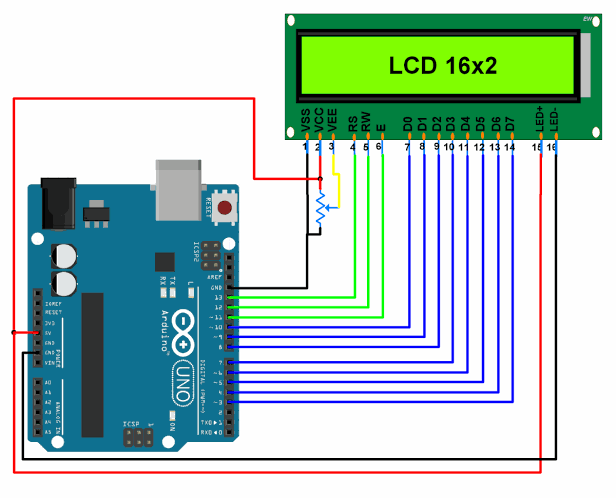
\includegraphics[width=0.35\textwidth]{connec.png}
	 \caption{\label{fig:Connections}}
 \end{figure}
\section{RESULTS}
Download the assembly code given in the link below and execute them to see the output as shown in Fig.4, where the output is displayed on the LCD screen.\\
 https:https://github.com/salad-12/FWC-INTERNSHIP/blob/main/assembly/codes/hello.asm
\begin{figure}[h] 
	\centering 
	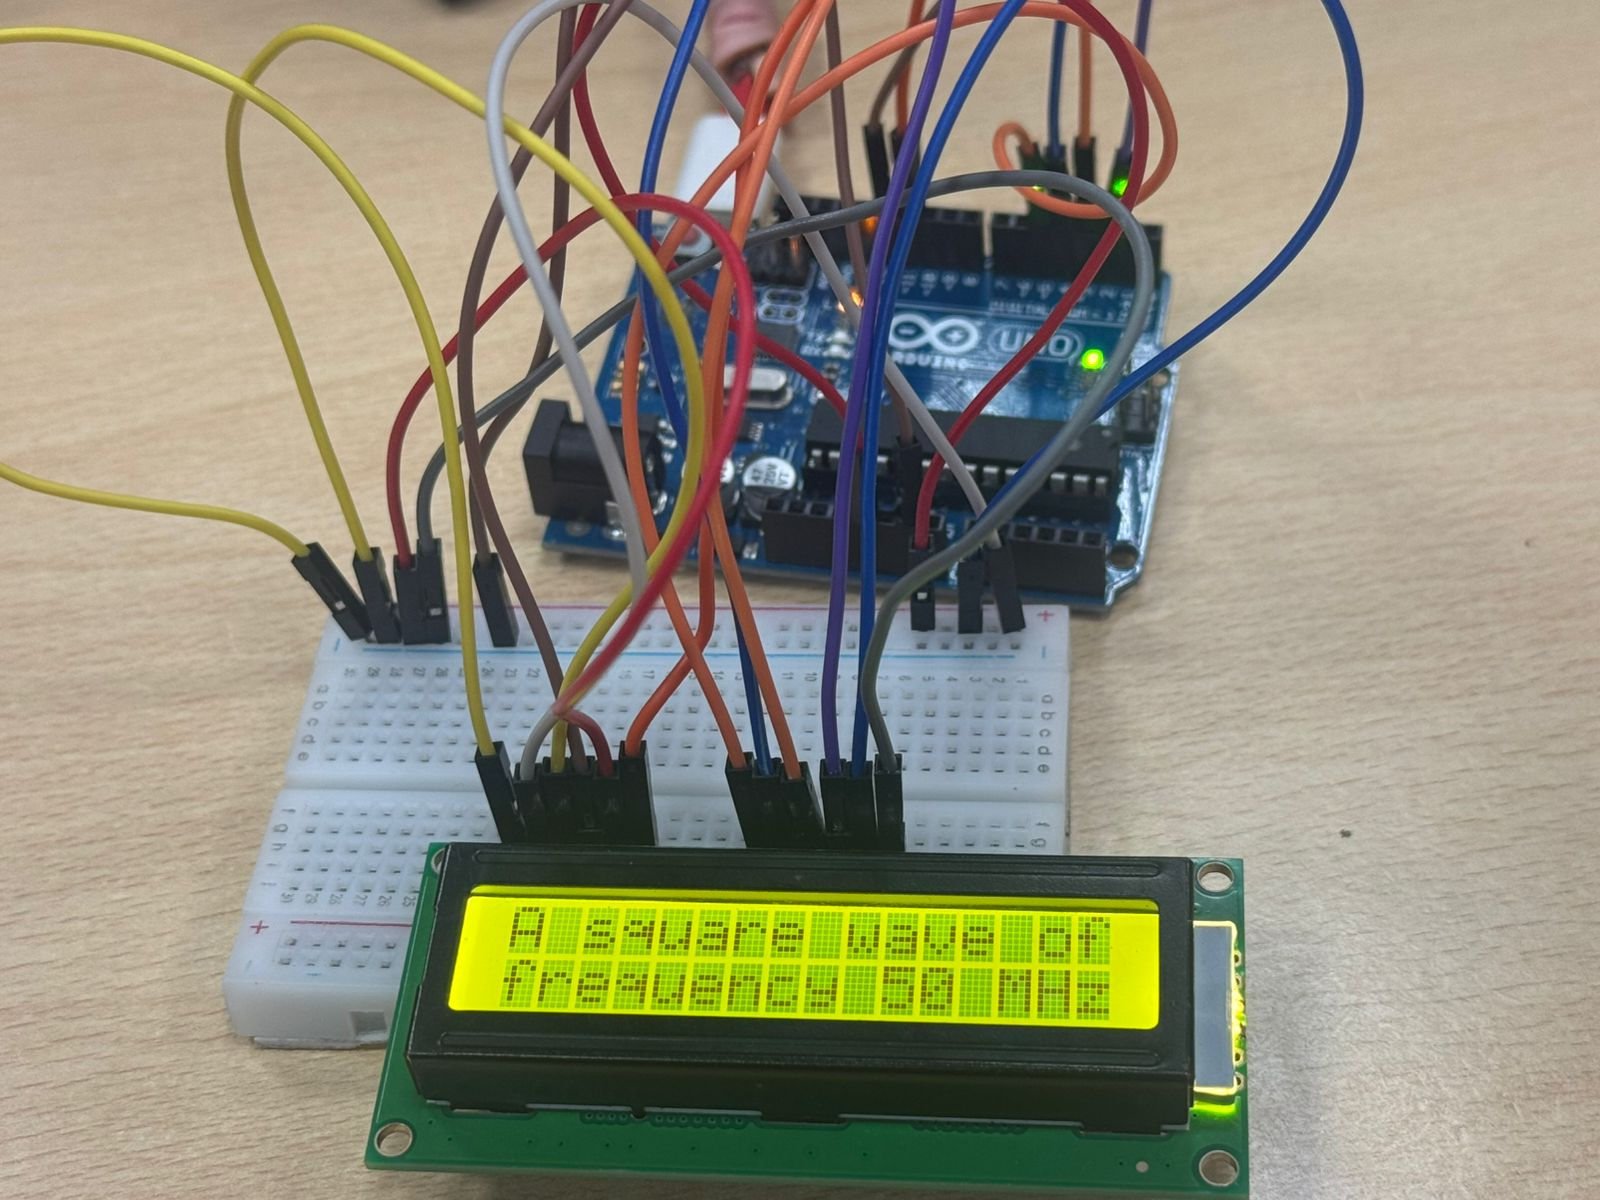
\includegraphics[width=0.4\textwidth]{assembly.jpg}
	\caption{\label{fig:Result}}    
\end{figure}
\section{CONCLUSION}
The MUX allows selection between two input signals based on a control signal, efficiently routing data to the desired output. The integration with an LCD provides a clear visualization of the output, enhancing user interaction and system monitoring. The assembly code was developed to manage both the multiplexer selection logic and LCD display operations, demonstrating effective hardware-software interfacing for embedded systems applications. This work highlights the use of low-level programming to control and interface digital components.
\end{document}
